\documentclass[a4paper,12pt]{article}
\usepackage{amsfonts}
\usepackage{tikz}
\usetikzlibrary{shapes.geometric}
\usetikzlibrary{arrows.meta,arrows}
\begin{document}

\title{Awkward State Machines}
\author{Will Dengler}
\maketitle

\section{Introduction}
Imagine you had a ball of yarn of infinite length and a pair of scizzors. Now choose some arbitrary length of yarn and cut it - we'll refer to this length as 1. Next, cut a second strand of yarn that has length 2 relative to your original piece of yarn and set it aside. Now, extend the yarn to length 3 and repeat the following instructions:
\begin{enumerate}
\item For every strand of yarn you have cut so far (other than the strand of length 1), check if the current extension of yarn can be split into even segments of the same length as the current strand by 'walking' the shorter strand up the longer one until you reach the end of or pass the end of the extended piece of yarn; if you reach the end of the extended piece exactly, then the extension can be divided into even segments. If none of the previous strands can be used to divide the current extension evenly, then double the length of the extended peice of yarn, then cut it in half, finally, set the cut strand aside with the others. Do not cut the extension if one of the previous strands does divide the extension evenly.
\item Using your strand of length 1, increase the length of the extension by 1.
\item Repeat the above two steps.
\end{enumerate} 

If you follow the above instructions, then order the strands of yarn you cut by their length, and finally wrote out their lengths relative to the strand of length 1, then you will find yourself writing down the prime numbers in consequetive order. The fact that this simple experiment derives the prime numbers using relative distance has always fascinated me. I've always had an itching notion that an algorithm based solely on relative distance, rather than integer arithmetic, would outperform the standard methods for discovering the primes in consequetive order. However, the problem of how to encode distance and divisibility without actually using numbers seemed to be impossible; after all, how do you tell a computer to use a ball of yarn and scizzors? And even if we could, the act of walking the strands up the extension is going to be pretty slow. 

Let's modify our experiment slightly to include tacks and a corkboard. Start again by cutting some length of yarn for defining length 1. Now, using your piece of yarn, seperate two tacks on your board 1 unit away from one another. You can now determine the strand of length two by wrapping your ball of yarn around the tacks such that you start at one tack, wrap around the second, and then return to the first tack, then cut the yarn to produce the strand of length two. Now use the strand of length two to place two more tacks in your board at 2 units apart.Now using the tacks for length 1, create a strand of length 3 and repeat the following instructions:   
\begin{enumerate}
\item For every pair of tacks on the board (other than the unit tacks), wrap the current extension of yarn around the tacks to check for divisibility. The extension is divisible if the yarn perfectly touches one of the tacks when it runs out of length. If none of the current pairs of tacks divide the extension evenly, then double the extension, cut it in half, and use the new strand to set apart a new pair of tacks on your board.
\item Use the unit pair of tacks to increase the length of the extension by 1.
\item Repeat the above two steps.
\end{enumerate} 

The above experiment is very simliar to the first. The pairs of tacks you've placed will wind up enumerating the primes once again. We are also still stuck with the problem of how could we encode this algorithm without integers, and the algorithm still isn't performing very quickly. However, the algorithm does highlight an important concept, our tacks use circles (technically ovals) in order to check the length of the extended piece of yarn. This is amazing because it allows us to check for divisiblity without counting anything out, instead, we just keep wrapping the yarn around until we get to the end; thus we don't need to know \textit{how} many times we've wrapped the yarn around, we just have to look where it winds up at the end.   

Let's modify our experiment once again. This time, you need tacks, a corkboard, and little flags that you can stick into the board (a needle with red tape for example). Start by placing two tacks down on the leftmost side of the board in a vertical line, and place a flag next to the bottom tack. Next, place three tacks in a vertical line to the right of those (imagine you are creating a bar graph with the tacks) and place a flag next to the highest tack. This expirement will require you to keep the vertical lines you create with the tacks distinct from one another, we shall refer to each line as a bar. Each bar in your board will always have a flag next to one of it's tacks. Repeat the following to run the experiment:
\begin{enumerate}
\item For every bar except the rightmost, move the flag to the tack above the one it is currently at; unless the flag is currently at the topmost tack in the bar, then move the flag to the bottom tack in the bar.
\item If there are no flags on any of the bottom tacks after you've moved every bar (other than the rightmost), then move the flag of the rightmost bar to its bottom tack and then create a new bar to the right of it that has one more tack than it, and place the new bar's flag at it's top tack.  
\item If there was a flag on one of the bottom tacks, then add a new tack to the top of the rightmost bar, and place it's flag next to the new tack.
\item Repeat the above three steps. 
\end{enumerate}

If you run the above experiment and then count the number of tacks in each bar, you will find that the number of tacks in the bars enumerate the prime numbers in consequetive order. How did this happen? Well, this experiment is much more similar to the last two than it first appears. In this case, the way we move the flags on each bar is the same as wrapping the extended piece of yarn around the tacks in experiment two, or 'walking' the yarn up the extended piece of yarn from experiment one. However, this time our flags our able to preserve the state from the last iteration since you just have to move the flags one tack forward. The moving of each tack can be done in constant time for each bar, and is incredibly fast relative to the time it takes to re-wrap the extended strand of yarn around the tacks, or perform the 'walks'. Furthermore, this expirement doesn't need distance; rather, it only needs relative position (bottom tack, tack above that, ..., tack below top tack, top tack). By replacing distance with relative position, we can easily encode our experiment without the use of numbers using cycle graphs implemented via linked lists. 
  
\section{Cycle Graphs}

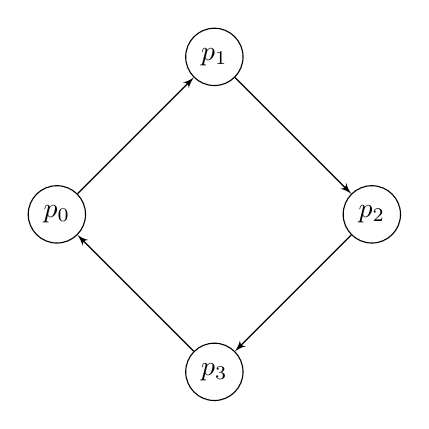
\begin{tikzpicture}

\tikzset{vertex/.style = {shape=circle,draw,minimum size=1.5em}}
\tikzset{edge/.style = {->,> = latex'}}

\node[vertex] (a) at  (0,0) {$p_0$};
\node[vertex] (b) at  (2,2) {$p_1$};
\node[vertex] (c) at  (4,0) {$p_2$};
\node[vertex] (d) at  (2,-2) {$p_3$};
%edges
\draw[edge] (a) to (b);
\draw[edge] (b) to (c);
\draw[edge] (c) to (d);
\draw[edge] (d) to (a);

\end{tikzpicture}\\
\\
\textbf{Definition}\\
A \textit{cycle graph} is a directed, connected graph whose points form a circle. More explicity, for any $n > 1$, the cycle graph $CG_n$ has points $\{$ $p_0, p_1, ..., p_{n-1}$ $\}$ such that for any $i < n - 1$, $p_i$ has only one edge which goes to $p_{i + 1}$, and $p_{n-1}$ has only one edge going to $p_0$.\\
\\ 
\\
\textbf{Lemma}\\
For any cycle graph $CG_n$, for any $p_i \in CG_n$, a walk of length $k = n - i$ will end at point $p_0$.\\
\\
\textit{Proof}\\
For any point $p_j \in CG_n$, there is only one edge that can be traversed, thus there is only one walk that can be made.\\
Furthermore, point $p_j$ is $h = n - j - 1$ steps from point $p_{n-1}$.\\
Thus, moving $k = h + 1 = n - j - 1$ steps from $p_j$ will land you on the point $p_{n-1}$ has an edge to, which is $p_0$ by defining of the cycle graph.\\
\textit{Q.E.D}\\ 
\\ 
\\
\textbf{Lemma}\\
For any cycle graph $CG_n$, a walk of length $n$ from $p_i$ will end at point $p_i$.\\
\\
\textit{Proof}\\
For any $p_i \in CG_n$, a walk of length $n - i$ will end at point $p_0$.\\
Thus, moving the final $j = n - (n - i) = i$ steps from point $p_0$ will land you on point $p_i$.\\
\textit{Q.E.D}\\
\\
\\
\textbf{Corollary}\\
For any cycle graph $CG_n$, a walk of length $kn$, $k > 0$, from $p_0$ will end at point $p_0$.\\
\\
\textit{Proof}\\
If we move $n$ steps from $p_i$ we will return to $p_i$ by the above.\\
Assume after moving $in$, $i \geq 1$ steps from $p_i$, you have returned to point $p_i$.\\
Then, moving $n$ more steps from there will again return to point $p_i$.\\
Thus moving $in + n = (i+1)n$ steps from $p_i$ returns you to $p_i$.\\
\textit{Q.E.D}\\
\\
\\
\textbf{Lemma}\\
For any cycle graph $C_n$, for any $k > 0$, for any $p_i \in C_n$, a walk of length $k$ starting at $p_i$ will end at point $p_j$ where $j = i + k$ $mod$ $n$.\\
\\
\textit{Proof}\\
Let $CG_n$ be at point $p_i$.\\
Let $0 > k$.\\
If $k > n$, then there exists $q \geq 0$ such that $qn + r = k$ with $0 \leq r < n$.\\
Furthermore, moving $qn$ positions from $p_i$ will return the cycle to $p_i$, leaving $r$ moves left.\\
\\
Let $e = i + r$.\\
Assume $e < n$, then moving $r$ positions from $p_i$ will land on $p_{i + r}$.\\
Thus, if $e < n$, moving $k = qn + r$ positions resulted in position $i + r = i + (qn + r)$ $mod$ $n = i + k$ $mod$ $n$.\\
\\
Assume $e \geq n$.\\
Then $e = n + a = i + r$ for $0 \leq a < n$.\\
Thus, $a = (i + r) - n = e - n$
\\
We can move $n - i$ positions from $p_i$ to return to point $p_0$.\\
Leaving $r - (n - i) = r - n + i$ = $(r + i) - n = e - n = a < n$ moves remaing.\\
Therefore, the cycle will land on point $p_a$.\\
\\
We need to show that $a = i + k$ $mod$ $n$.\\
Substituting give us:\\
\\
$i + k$ $mod$ $n = i + (qn + r)$ $mod$ $n = i + r$ $mod$ $n$\\ 
$= e$ $mod$ $n = (n + a)$ $mod$ $m = a$ $mod$ $m$.\\ 
\\
Thus we have shown that moving $k$ steps from $p_i$ will result in point $p_j$ where $j = k + i$ $mod$ $n$.\\
\textit{Q.E.D}
\section{Activation Cycle Machines}

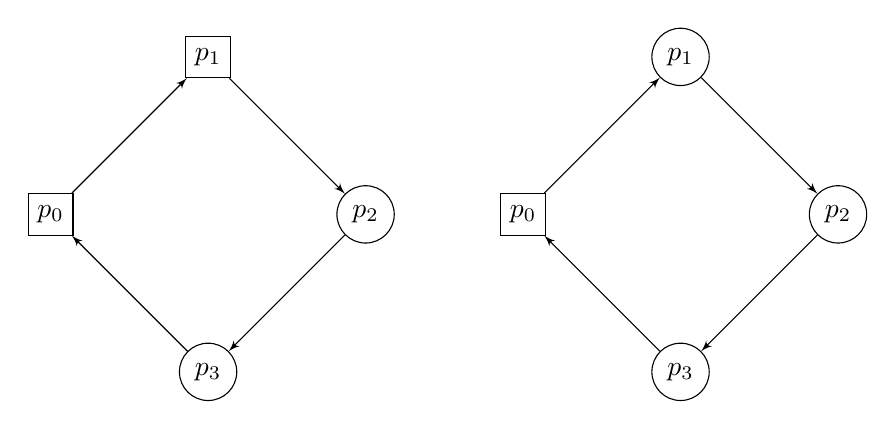
\begin{tikzpicture}

\tikzset{vertex/.style = {shape=rectangle,draw,minimum size=1.5em}}
\tikzset{edge/.style = {->,> = latex'}}

\node[vertex] (a) at  (0,0) {$p_0$};
\node[vertex] (b) at  (2,2) {$p_1$};
\tikzset{vertex/.style = {shape=circle,draw,minimum size=1.5em}}
\node[vertex] (c) at  (4,0) {$p_2$};
\node[vertex] (d) at  (2,-2) {$p_3$};

\draw[edge] (a) to (b);
\draw[edge] (b) to (c);
\draw[edge] (c) to (d);
\draw[edge] (d) to (a);

\tikzset{vertex/.style = {shape=rectangle,draw,minimum size=1.5em}}
\node[vertex] (a1) at  (6,0) {$p_0$};
\tikzset{vertex/.style = {shape=circle,draw,minimum size=1.5em}}
\node[vertex] (b1) at  (8,2) {$p_1$};
\node[vertex] (c1) at  (10,0) {$p_2$};
\node[vertex] (d1) at  (8,-2) {$p_3$};

\draw[edge] (a1) to (b1);
\draw[edge] (b1) to (c1);
\draw[edge] (c1) to (d1);
\draw[edge] (d1) to (a1);

\end{tikzpicture}\\
\\
\textbf{Definition}\\
An \textit{activation cycle machine} (ACM) is state machine that runs on top of a cycle graph $CG_n$, that has been equipped with a subset of $0 < a < n$ activator points $A = \{$ $p_i$ $|$ $0 \leq i < a < n$ $\}$.\\
\\
Each state of an ACM is associated with a position $p \in CG_n$.\\
The initial state (state $0$) of any ASM has position $p_0 \in CG_n$.\\
\\
If the position of an ACM is $p_j$ on state $i - 1$, then the position at state $i$ will be the point connected to by $p_j$.
Thus, if $j < n - 1$, then the next state's position will be $p_{j+1}$; otherwise, if $j = n - 1$, then the next state's position will be $p_0$.\\
\\
We denote the ACM containing cycle graph $CG_n$ and $a$ activator nodes as $C_{n,a}$.\\
\\
For simplicity, if the current position of $C_{n,a}$ is $p_i$ on state $j$, we write $\overline{C}^j_{n,a} = i$.\\ 
\\
If the current position of an ACM, $C_{n,a}$ is within the set of activotors ($\overline{C}_{n,a} < a$), then we say the ACM is \textit{active}; otherwise, we say the ACM is \textit{inactive}.\\
\\
\\
\textbf{Theorem}\\
For any ACM, $C_{n,a}$, for any state, $k$, the position of state $(k + i)$ is given by taking a walk of length $i$ starting at position $\overline{C^k}$ around $CG_n$, thus the position of state $k + i$ is: $\overline{C^k} + i$ $mod$ $n$.\\
\\
\textit{Proof}\\
By defininiton of an ACM, if the position of an ACM is $p_j$ on state $i - 1$, then the position at state $i$ will be the point connected to by $p_j$, which is equivalent to taking a walk of length 1 on $CG_n$ starting on point $p_j$.\\
\\
Assume for some $j$, $1 \leq j \leq i$, that the position of state $k + j$ is given by taking a walk of length $j$ starting at position $\overline{C^k}$ around $CG_{n,a}$.\\
\\
Then the position on state $k + j$ is given by $\overline{C^k} + j$ $mod$ $n$.\\
Thus, the the next state's position will be given by $\overline{C}^{k + j + 1} = \overline{C^k} + j + 1$ $mod$ $n$, which is the end position of a walk of length $j + 1$ when starting at point $\overline{C^k}$ on $CG_{n,a}$.\\
\textit{Q.E.D}\\
\\
\\
\textbf{Corollary}\\
The position of $C_{n,a}$ on state $k$ is given by $k$ $mod$ $n$.\\
\\
\textit{Proof}\\ 
The initial state, $0$, starts at position $0 = 0$ $mod$ $n$.\\
Thus the position of state $k = k + 0$ is given by:\\
$|C^0| + k$ $mod$ $n = 0 + k$ $mod$ $n = k$ $mod$ $n$.\\
\textit{Q.E.D}\\   
\\
\\
\textbf{Corollary}\\
$C_{n,a}$ is active on state $k$ if and only if $k$ $mod$ $n < a$.\\
\\
\textit{Proof}\\
An ACM, $C_{n,a}$ is active if and only if it's position is on one of it's activators.\\
The activators of $C_{n,a}$ are defined to be $p_{0 \leq i < a}$, or equivalenty positions $0 \leq i < a$.\\
\\
Thus, an $C_{n,a}$ is only active if it's position is less than $a$.\\
Thus, $C$ is active if and only if $a > \overline{C^k} = k$ $mod$ $n$.\\
\textit{Q.E.D} 
  
\section{Awkward State Machines}

Now that we have our definitions for cycle graphs and ACMs, we are almost ready to formally define the \textit{awkward state machine} or \textit{ASM}. An ASM is a state machine for the purpose of generating a set of ACMs using a pre-existing set of ACMs. In order to accomplish this task, with each step of an ASM, all the pre-existing ACMs state's are incremented by one; if none of the ACMs are active after moving, then a new ACM is added to the ASM and it's position is set to 0. Thus, every state of an ASM has at least one ACM that is active.\\
\\
Every ASM starts with an initial ACM set to position 0, and an \textit{activation branch} of length one greater than the ACM. An activation branch is simply an ACM that has the edge removed from its last point to its inital point; thus an activation branch forms a line instead of a circle. Whenever the ASM must create a new ACM, it does so by creating a copy of its activation branch, then adds the missing edge to the original branch in order to form the new ACM required by the machine.  Furthermore, a new node is added to the end of the copied activation branch. If the ASM does not need to create a new ACM after moving, then a new node is added to the end of its activation branch. Thus, the length of an ASM's activation branch increases by one with every iteration.\\
\\
This section will explore several fundamental questions about ASMs and the sets of ACMs they generate. We will find that the sets of ACMs generated by ASMs have a unique and unexpected relationship to modular arithmetic. For instance, we will see that the most basic ASM generates the prime numbers; and all other ASMs generate sets of integers just as strange, or awkward, as the primes. Furthermore, in our final theorem of this section, we will show that every ASM will generate an infinite set of ACMs if left running.\\   
\\
We will begin this section by formally defining the activation branch and proving that we can indeed create an ACM by adding an edge to it. From there, we will formally define ASMs and then begin our exploration.\\
\\
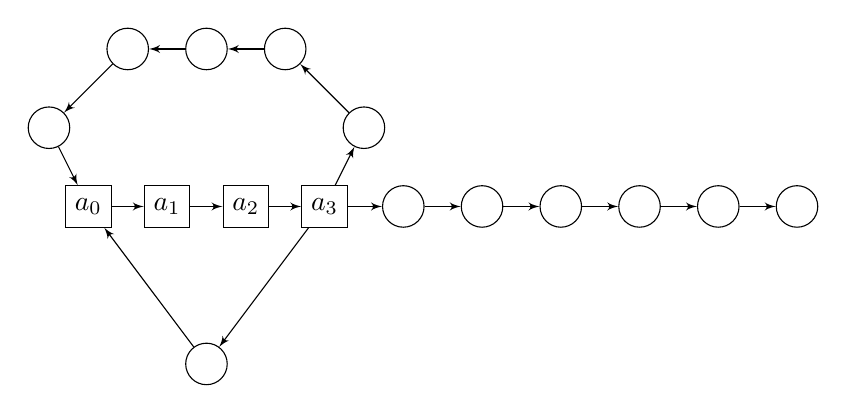
\begin{tikzpicture}

\tikzset{vertex/.style = {shape=rectangle,draw,minimum size=1.5em}}
\tikzset{edge/.style = {->,> = latex'}}

\node[vertex] (a0) at  (0,5) {$a_0$};
\node[vertex] (a1) at  (1,5) {$a_1$};
\node[vertex] (a2) at  (2,5) {$a_2$};
\node[vertex] (a3) at  (3,5) {$a_3$};
\tikzset{vertex/.style = {shape=circle,draw,minimum size=1.5em}}
\node[vertex] (b0) at  (1.5,3) {};

\node[vertex] (c0) at  (3.5,6) {};
\node[vertex] (c1) at  (2.5,7) {};
\node[vertex] (c2) at  (1.5,7) {};
\node[vertex] (c3) at  (0.5,7) {};
\node[vertex] (c4) at  (-0.5,6) {};

\node[vertex] (d0) at  (4,5) {};
\node[vertex] (d1) at  (5,5) {};
\node[vertex] (d2) at  (6,5) {};
\node[vertex] (d3) at  (7,5) {};
\node[vertex] (d4) at  (8,5) {};
\node[vertex] (d5) at  (9,5) {};

\draw[edge] (a0) to (a1);
\draw[edge] (a1) to (a2);
\draw[edge] (a2) to (a3);

\draw[edge] (a3) to (b0);
\draw[edge] (b0) to (a0);

\draw[edge] (a3) to (c0);
\draw[edge] (c0) to (c1);
\draw[edge] (c1) to (c2);
\draw[edge] (c2) to (c3);
\draw[edge] (c3) to (c4);
\draw[edge] (c4) to (a0);

\draw[edge] (a3) to (d0);
\draw[edge] (d0) to (d1);
\draw[edge] (d1) to (d2);
\draw[edge] (d2) to (d3);
\draw[edge] (d3) to (d4);
\draw[edge] (d4) to (d5);

\end{tikzpicture}\\
\\
\textbf{Definition}\\
An \textit{activation branch} is directed graph that forms a line. Explicity, the activation branch of length $n$ has points $\{$ $p_0, p_1 ..., p_{n-1}$ $\}$ such that for every point $p_{i < n -1}$ has a single edge connecting it to $p_{i+1}$, and $p_{n-1}$ does not have any edges extending from it.\\
\\
Furthermore, an activation branch is equipped with $a > 0$ activator points: $A = \{$ $p_i$ $|$ $0 \leq i < a < n$ $\}$.\\ 
\\
We denote the activation branch with length $n$ and $a$ activator nodes $B_{n,a}$.
\\
\\
\textbf{Lemma}\\
For any $B_{n,a}$, adding an edge extending from $p_{n-1}$ to $p_0$ produces the cycle graph $CG_n$ for ACM $C_{n,a}$.\\
\\
\textit{Proof}\\ 
By definition of $B_{n,a}$, all points $p_{i < n -1}$ have the same edges as the first $n - 1$ points in $CG_n$ for ACM $C_{n,a}$.\\
\\
Furthermore, the first $a$ points of $B_{n,a}$ are it's activator points, which are the activators of $C_{n,a}$.\\
\\
Thus, the only edge missing from $B_{n,a}$ that is contained within $CG_n$ is from  $p_{n-1}$ to $p_0$.\\
\\
Therefore, adding the edge will convert $B_{n,a}$ into $CG_n$ for $C_{n,a}$.\\
\textit{Q.E.D}\\
\\
\textbf{Definition}\\
An \textit{awkward state machine} (ASM) is state machine running on top of a directed graph composed of a set of ACMs and a single activation branch.\\
\\
Every ASMs initial state contains a single $ACM$, $C_{m,a} = C_0$, and the activation branch, $B_{m+1,a}$.\\
Furthermore, the position of $C_0$ on the initial state is $0$.\\
We denote the ASM with an initial state containing $C_{m,a}$ as $S_{a,n=m-a}$.\\
\\
To progress from state $i - 1$ to state $i$ for ASM, $S$, first move every ACM in $S$ to it's next state.\\
If none of the ACMs in $S$ are active after moving to their next state, then:
\begin{enumerate}
\item Create a copy of the activation branch, giving you branches $B$ and $B`$.
\item Convert $B$ into an $ACM$, $C$, by adding an edge to it's last point, thus leaving a single activation branch $B`$. Set the position of $C$ to $0$. Now $C$ is contained within the set of ACMs for $S$.
\end{enumerate}
Regardless of whether one of the ACMs were active, add a new point to the end of the activation branch. Explicitly, if the activation branch had length $n$, then add an edge extending from $p_{n-1}$ to the new point $p_n$, thus creating an activation branch of length $n + 1$.\\
\\
If none of the ACMs were active after moving them to their next state, we say that $S$ is \textit{inactive} after moving; otherwise we say $S$ is \textit{active} after moving. Therefore, we only add a new ACM to $S$ when $S$ is inactive after moving.\\
\\
We denote the inition cycle of an ASM $C_0$, the first discovered cycle $C_1$, and the $n$th discovered cycle $C_n$.\\
\\
We denote the graph of ASM $S_{a,n}$ on state $k$ as $S^k$.\\
\\
If $C_{p,a}$ is discovered by ASM $S_{a,n}$ on some step $k$, then we say that $C_{p,a}$ is \textit{discoverable} by $S$.\\
\\
\textbf{Definition}\\  
We'll define $[S^a] = \{$ $C_i$ within the graph of $S$ on step $a$ $\}$,\\
and $[S] = \{$ $C_0$ and all $C_i$ disoverable by $S$ $\}$. We refer to $[S]$ as the \textit{school} of cycles for $S$.\\
\\
\\
\textbf{Lemma}\\
For $S_{a,n}$, the length of the branch, $B$, on step $k$ is given by $|B^k| = k + a + n + 1$.\\
\\
\textit{Proof}\\  
One step $0$, the length of branch $B$ is given by $|B^0| = 0 + a + n + 1$.\\
With each step, a single node is added to the branch $B$. Thus, $|B^{i+1}| = |B^{i}| + 1$.\\
\\
Assume $|B^{i}| = i + a + n + 1$.\\
Then $|B^{i+1}| = |B^{i}| + 1 = (i + a + n + 1) + 1 = (i + 1) + a + n + 1$.\\
\\
Thus we have shown that $|B^k| = k + a + n + 1$ by induction.\\
\textit{Q.E.D}\\
\\
\\
\textbf{Lemma}\\
For $S_{a,n}$, if $C_i$ is discovered on step $k$, then the length of $|C_i| = |B^{k-1}| = k + a + n$.\\
\\
Assume for $S_{a,n}$, that $C_i$ is discovered on step $k$.\\
\\
To produce state $k$, the ASM algorithm first moved all $C_j$ for $j < i$ from state $C^{k-1}$ to state $C^k$. After doing so, there did not exist a $j < i$ such that $C_j$ was active. Therefor, the algorithm copied the branch $B^{k-1}$ and closed one of the two branches to create $C_i$.\\
\\ 
Thus, the length of $C_i$ is equal to the length of the branch $B^{k-1}$:\\ $|C_i| = |B^{k-1}| = (k - 1) + a + n + 1 = k + a + n$.\\
\textit{Q.E.D}\\
\\
\\
\textbf{Lemma}\\
For $S_{a,n}$, $|C_{i}| \geq |C_{i-1}| + a$.\\
\\
\textit{Proof}\\  
Assume cycle $C_i$ is discovered by $S_{a,n}$ on step $k$.\\
\\
Then $\overline{C^k_i} = 0$.\\
Furthermore, the new branch, $B$, will have $|C_i| + 1$ nodes at step $k$.\\
\\
For next, $1 \leq j < a$ steps, the cycle  $C^{k+j}_i$ will be active since there are $a$ activation nodes.\\
Furthermore, the length of the branch $B$ at each step will be given by $|B| = |C_i| + j + 1$.\\
\\
The $a$th step after discovering $C_i$ will be the first time that $C_i$ will be inactive. The branch length of the $(a-1)$th step is given by $|B^{j + a - 1}| = |C_i| + a$. Thus, if $C_p$ for $0 \leq p < i$ are also inactive on step $a$th step after discovering $C_i$, then we will have to close $B$ on the $a$th step, thus creating cycle $C_{i+1}$ with length $|C_{i+1}| = |B^{j + a - 1}| = |C_i| + a$. Furthermore, if any of the cycles $C_p$ were active on the $a$th step after discovering $C_i$, then the branch would not close, thus the next cycle's length is at least as long as the branch on the $(j+a)$th step: $|C_{i+1}| >= |B^{j + a}| = |C_i| + a + 1$.\\
\\
Thus, we have shown that  $|C_{i}| \geq |C_{i-1}| + a$.\\
\textit{Q.E.D}\\
\\
\\
\textbf{Lemma}\\
For any $C_i, C_j \in [S_{a,n}]$ with $j < i$, it holds that $|C_{i}| \geq |C_j| + (i - j)a$.\\
\\
\textit{Proof}\\ 
If $i = j + 1$, then $j - i = 1$.\\
Thus, $|C_i| \geq |C_j| + a = |C_j| + (j - i)a$.\\
\\
Assume for $k$, $i < k \leq j$, that $|C_k| \geq |C_i| + (k-i)a$.\\
\\
Then $|C_{k+1}| \geq |C_k| + a \geq (|C_i| + (k-i)a) + a = |C_i| + (k + 1 - i)a$.\\
\\
Thus we have shown that $|C_{i}| \geq |C_j| + (i - j)a$ by induction.\\
\textit{Q.E.D}\\
\\
\\
\textbf{Corollary}\\
For any cycle $C_{j}$ of an ASM, $S_{a,n}$, $C_j$ has at least $n + ja$ non-activator nodes.\\
\\
\textit{Proof}\\
$C_0$ is defined to have $n$ activator nodes.\\
\\
Let $C_{j>0} \in [S_{a,n}]$.\\
\\
Then $|C_j| \geq |C_1| + (j-1)a \geq (|C_0| + a) + (j-1)a $\\
$= (2a + n) + (j-1)a = n + (j+1)a$.\\
\\
Thus, after removing the $a$ activator nodes from $C_j$, there are at least $n + ja$ non-activator nodes left.\\
\textit{Q.E.D}\\
\\
\\
\textbf{Lemma}\\
Every ASM discovers at least one cycle.\\
\\
\textit{Proof}\\
Let $C_0$ by the initial cycle for ASM, $S_{a,n}$.\\
\\
After taking $a$ steps from the initial state of the $S$, the ASM will be on it's first non-activator node.\\
\\
Since $C_0$ is the only cycle, the ASM would be inactive, thus a new cycle would be created.\\
\textit{Q.E.D}\\
\\ 
\\
\textbf{Lemma}\\
For any step, $k$, for any $C_i \in [S^k_{a,n}]$, it holds that $\overline{C^k_i} = (k + a + n)$ $mod$ $|C_i|$.\\
\\
\textit{Proof}\\  
The initial cycle $C_0$ starts at position $0$ on step $0$. By properties of ACM's, we know that the position of $C_0$ is given by:\\
\\
$\overline{C^k_0} = k$ $mod$ $|C_0| $
$= [k +(a + n)]$ $mod$ $(a + n)$
$= (k + a + n)$ $mod$ $|C_0|$.\\
\\
If a cycle, $C_i$, is discovered on step $k$, then we know it's length is given by $|C_i| = k + a + n$. Furthermore, when it's dicovered, it's position is set to 0.\\
\\
Thus, the position of $C^k_i$ is given by:\\
\\
$\overline{C^k_i} = 0 = (k + a + n)$ $mod$ $(k + a + n) = (k + a + n)$ $mod$ $|C_i|$.\\
\\
By properties of ACM's, the position for all steps $j > k$ will be given by:\\
\\
$\overline{C^j} = (\overline{C^k} + (j - k))$ $mod$ $|C^i|$
$= (0 + (j-k))$ $mod$ $(k + a + n)$\\
$= (k + a +n) + (j-k)$ $mod$ $|C_i| $
$= (j + a + n)$ $mod$ $|C_i|$.\\
\\
Therefor we have shown that the position of $C_i$ on step $k$ for any $C_i \in [S^k_{a,n}]$ is given by $\overline{C^k_i} = (k + a + n)$ $mod$ $|C_i|$ for any $C_i$ in $[S^k]$.\\
\textit{Q.E.D}\\
\\
\\
\textbf{Corollary}\\
For any cycle $C_j \in [S_{a,n}]$, moving $k|C_j|$ steps will maintain $C_j$'s position.\\
\\
\textit{Proof}\\
Let $C_j \in [S]$.\\
Assume $S$ is on step $p$.\\
\\
Then $\overline{C_j} = p + a + n $ $mod$ $|C_j|$.\\
Thus, if we move $k|C_j|$ steps from $p$, the position of $C_j$ will be given by:\\
\\
$p + a + n + k|C_j|$ $mod$ $|C_j| = p + a + n$ $mod$ $|C_j|$.\\
\\
Therefor $C_j$'s position was maintained.\\
\textit{Q.E.D}\\
\\
\\
\textbf{Lemma}\\
For any cycle $C \in [S]$, if $k \geq |C|$, then the position of $C$ after moving $k$ steps from $C$'s discovery is the same as moving $k$ $mod$ $|C|$ steps.\\
\\
\textit{Proof}\\
Assume $C \in [S]$, and $S$ is on step $p$.\\
Then the position of $C$ is given by $p + a + n$ $mod$ $|C|$.\\
\\
Let $k > |C|$, $b = k$ $mod$ $|C|$.\\
\\
The position of $C$ on step $p + k$ is given by:\\
$p + k + a + n$ $mod$ $C = p + b + a + n$ $mod$ $C$ which is the position after moving $b$ steps from $p$.\\
\textit{Q.E.D}\\
\\
\\
\textbf{Lemma}\\
For any $C_i, C_j \in [S_{a,n}]$ with $j < i$, it holds that $|C_i|$ $mod$ $|C_j| \geq a$.\\
\\
\textit{Proof}\\  
Assume for ASM, $S_{a,n}$, that ACM, $C_i$, is discovered on step $k$.\\
\\
Then $|C_i| = k + a + n$.\\
We know also know that the position of $C^k_j$ must be greater than or equal to $a$; otherwise, $C_j$ would be active on step $k$ and we would not have discovered $C_j$.\\
\\
Furthermore, we know the position of $C^k_j$ is given by:\\
$\overline{C^k_j} = (k + a + n)$ $mod$ $|C_j|$.\\ 
\\
Finally, subsitituting gives us: $\overline{C^k_j} = |C_i|$ $mod$ $|C_j| \geq a$.\\
\\
Thus we have shown that, $|C_i|$ $mod$ $|C_j| \geq a$.\\
\textit{Q.E.D}\\ 
\\
\\
\textbf{Lemma}\\
For any $C_i \in [S_{a,n}]$, $|C_i|$ is the least positive integer greater than $|C_{i-1}|$ such that $|C_i|$ $mod$ $|C_j| \geq a$ for all $j < i$.\\
\\
\textit{Proof}\\
Assume you discovered $C_{i-1}$ on step $p$.\\
Assume $k$ is the first step after discovering $C_{i-1}$ such that all cycles are inactive (if we can show that cycle $C_i$ is discovered on step $k$, then our proof will be complete).\\
\\
Then, on all steps, $q$, $p \leq q < k$, there must exist at least one cycle $C_j$ that is active (implying $q + a + n$ $mod$ $|C_j| < a$). Therefore, the ASM algoirthm cannot create cycle $C_i$ on any step $p \leq q < k$.\\
\\
Furthermore, on step $k$, the algorithm must create $C_i$, giving us $\overline{C^k_i} = 0 = k + a + n$ $mod$ $|C_i|$.\\
\\
Thus, since $k + a + n = |C_i|$ is the least positive integer such that $|C_i|$ $mod$ $|C_j| \geq a$ for all $j < i$, and have proved our lemma.\\
\textit{Q.E.D}\\
\\
\\
\textbf{Definition}\\
A positive integer is prime if it's only factors are 1 and itself.\\
\\
\textbf{Axiom}\\
The $i$th prime number, $p_i$, is the least integer that is greater than the $(i-1)th$ prime number and is not divisible by $p_j$ for all $j < i$ (with the first prime number $p_0=2$).\\ 
Note: This is only an axiom because proving the statement is distracting to ASMs.\\
\\
\\
\textbf{Lemma}\\
$|S_{1,1}| = P = \{$ the set of prime numbers $\}$\\
\\
\textit{Proof}\\
$S_{1,1}$ starts with an initial cycle of length $1 + 1 = 2$, thus giving us the first prime number.\\
\\
For all $i, j$ such that $i > j \geq 0$, $C_i$ will have the property that $|C_i|$ $mod$ $|C_j| \geq 1$, equivalenty, $|C_i|$ is not divisible by any of the previous lengths $|C_j|$. Furthermore, $|C_i|$ is the smallest such integer greater than $|C_{i-1}|$ with the property of not being divisible by the previous cycle lengths.\\
\\
Thus, by our axiom, $S_{1,1}$ produces the prime numbers.\\
\textit{Q.E.D}\\ 
\\
\\
\textbf{Theorem}\\
For every ASM, $S$, the set $[S]$ is non-finite.\\
\\
\textit{Proof}\\  
Assume there exists an ASM, $S_{a,n}$ such that $[S_{a,n}]$ is finite.\\
Let $s$ be the number of cycles in $[S_{a,n}]$.\\
\\
Then there exists some step $p$ on which the last cycle, $C_{max}=C_{s-1}$ of the ASM is discovered.\\
\\
We know $C_{max}$ must have at least $n + (s-1)a > (s-1)a$ non-activator nodes.\\
\\
We also know that on step $p$, all cycles $C_{i<s}$ must have been inactive to have discovered $C_{max}$.\\
\\
Furthermore, on step $j$, $C_{max}$'s position is at 0.\\
\\
Let $z = \prod_{i<s}|C_i|$.\\
\\
If we move the $ASM$ $z$ steps, then the position of every $C_{i<z}$ will be maintained since $z$ is a multiple of the length of every $C_{i<z}$.\\
\\
Thus, if after moving $z$ steps from $p$, $C_{max}$ is inactive, then we would need to create a new cycle, and we'd be finished with our proof.\\
\\
Assume $C_{max}$ was active after moving the $z$ steps.\\
\\
Let $n =\overline{C_{max}}$\\
\\
We know $n < a$ since $C_{max}$ is inactive.\\
\\
Note: the position of $C_{max}$ after moving $zt$ steps is the same as after moving $nt$ steps since $z > |C_{max}|$ (if z were less than $|C_{max}|$, then moving $z$ steps would have inactivated $C_{max}$ since $z > a$).\\
\\
Let $j$ be the greatest integer such that $jn < a$.\\
Then your position after moving $jz$ steps will be $a - jn$.\\
Thus, the $(j+1)z$th step will put $C_{max}$ at position $(a-jn)+n \geq a$.\\   
\\
If the $ASM$ is to remain active, then $(a-jn)+n$ must go beyond all $(s-1)a$ non-activator nodes in $C_{max}$.\\
\\
Thus, $(a-jn)+n > a + (s-1)a \geq sa \geq 2a$.\\
\\
But both $n$ and $(a-jn)$ are less then $a$.\\
But that means: $a + a = 2a > (a-jn)+n \geq 2a$, which is a contradiction!\\
\\
Therefore, moving $(j+1)z$ steps from the discovery of $C_{max}$ will maintain the (inactive) positions of all $C_{i<z}$ and also move $C_{max}$ into one of it's inactive nodes, requiring a new cycle to be made, and completing our proof.\\
\textit{Q.E.D}\\   
\\
\\
\textbf{Corollary}\\
There are an infinite number of prime numbers.\\
\\
\textit{Proof}\\ 
$S_{1,1}$ produces the prime numbers, and $[S_{1,1}]$ is non-finite by the above theorem.\\
\textit{Q.E.D}

\textbf{Question}\\
For any two ASMs, are their schools unique?

\section{Needy Cycle Machines}

\textbf{Definition}\\
A \textit{Needy Cycle Machine} (NSM) is state machine running on top of a directed graph composed of a set of ACMs and a single activation branch.\\
\\
A NSM starts with $k > 0$ initial cycles, $\{$ $C_0, ..., C_{k-1}$ $\}$ . Each of the $k$ initial cycles must have a unique length and contain the same number of activator nodes. Futhermore, the initial position of every initial cycle is $0$.
\\
The initial branch length is a single node longer than the longest initial cycle.\\
\\
Like an ASM, every cycle in an NSM is moved one state with each iteration. However, an NSM is \textit{active} only if at least $k$ cycles are active; otherwise, the NSM is \textit{inactive}.\\
\\
If an NSM is inactive after moving all of it's cycles, then it behaves exactly as an ASM by copying its activation branch and creating a new cycle with one of the two branches.\\
\\
Regardless of whether an NSM is active after moving all of it's cycles, a new node is added to the end of the activation branch.\\
\\
\\
\textbf{Question}\\
Does every NSM discover an infinite number of cycles?\\
\\
\\
\textbf{Question}\\
What numbers do NSMs discover?

\section{Complicated Cycle Machines}

\textbf{Definition}\\
A \textit{Complicated Cycle Machine} (CCM) is basically the same as an ASM; however, the activators nodes of an CCM can be any of the nodes within the initial cycle, with the condition that position $0$ is always one of the activator nodes.\\
\\
\\
\textbf{Question}\\
Does every CSM discover an infinite number of cycles?\\
\\
\\
\textbf{Question}\\
What numbers do CSMs discover?

\end{document}